% Chapter 1

\chapter{Gesture recognition in the cultural heritage scenario}

\lhead{Chapter 4. \emph{Hand gesture recognition}} % This is for the header on each page - perhaps a shortened title

%----------------------------------------------------------------------------------------
Having presented our hand segmentation approach, we move a step forward and introduce a more complex problem: detecting static and dynamic hand gestures. As we said in the introductory chapter, the target scenario of our research is the cultural heritage domain. In fact, our goal is to deploy new gesture-based human machine interfaces to enhance museum experience.

In this chapter we provide algorithms that perform gesture analysis to recognize user interaction with artworks. We also propose to use scalable and distributed wearable devices capable of communicating with each other and with a central server. In particular the connection with the central server allows our wearable devices to grab gestures of past visitors for improving gesture analysis accuracy.

The proposed gesture recognition algorithm is compared to the current state of the art on benchmark datasets showing superior performance, and is tested in real and virtual museum environments. We further demonstrate that our gesture recognition approach can achieve acceptable accuracy results even with a few training samples performed by the visitor, and can benefit from distributed training in which gestures performed by other visitors are exploited.


\section{Proposed Method}
To our knowledge, the study of gesture recognition in the ego-centric paradigm has not yet been addressed. Even though not related to ego-vision domain, several approaches to gesture and human action recognition have been proposed. Sanin \etal \cite{sanin2013spatio} developed a new and more effective spatio-temporal covariance descriptor to classify gestures in conjunction with a boost classifier. Lui \etal \cite{lui2010action, lui2011tangent} used tensors and tangent bundle on Grassmann manifolds to classify human actions and hand gestures. Kim \etal \cite{kim2009canonical} extended Canonical Correlation Analysis to measure video-to-video similarity to represent and detect actions in video. However, all these approaches are not appropriate for the ego-centric perspective, as they do not take into account any of the specific characteristics of this domain, such as fast camera motion and background cluttering.
\begin{figure}
\centering
\subfigure{
                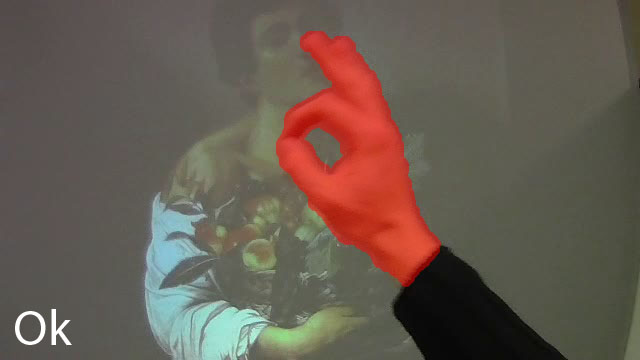
\includegraphics[width=0.23\textwidth]{Figures/ok_7141_7164_text16.jpg}
                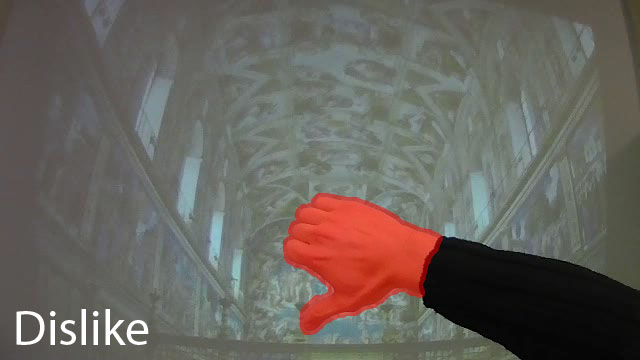
\includegraphics[width=0.23\textwidth]{Figures/dislike_3941_3969_text16.jpg}
} \\
\subfigure{
	    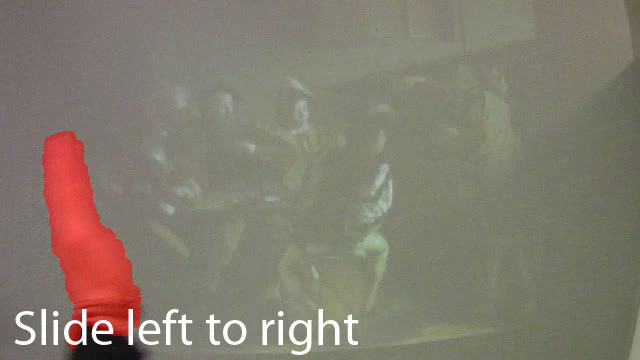
\includegraphics[width=0.23\textwidth]{Figures/slide_2_7438_7451_text5.jpg}
                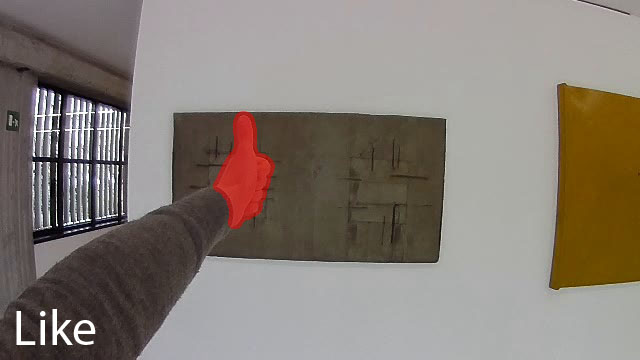
\includegraphics[width=0.23\textwidth]{Figures/like_7038_7080_text23.jpg}
} \\
\subfigure{
                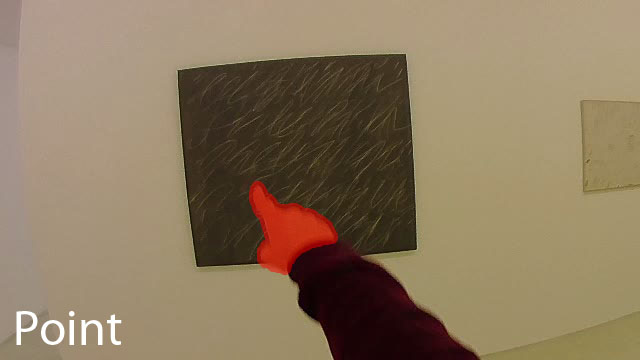
\includegraphics[width=0.23\textwidth]{Figures/point_15476_15505_text5.jpg}
                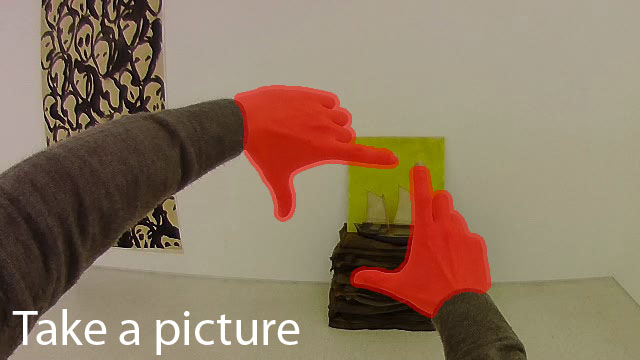
\includegraphics[width=0.23\textwidth]{Figures/take_a_picture_18622_18673_text37.jpg}
} \\
\caption{Results from the proposed hand segmentation and gesture recognition algorithms. Hand segmentation results are highlighted in red and detected gestures are reported in the bottom part of each frame.}
\label{sample}
\end{figure}

\begin{figure}
\centering
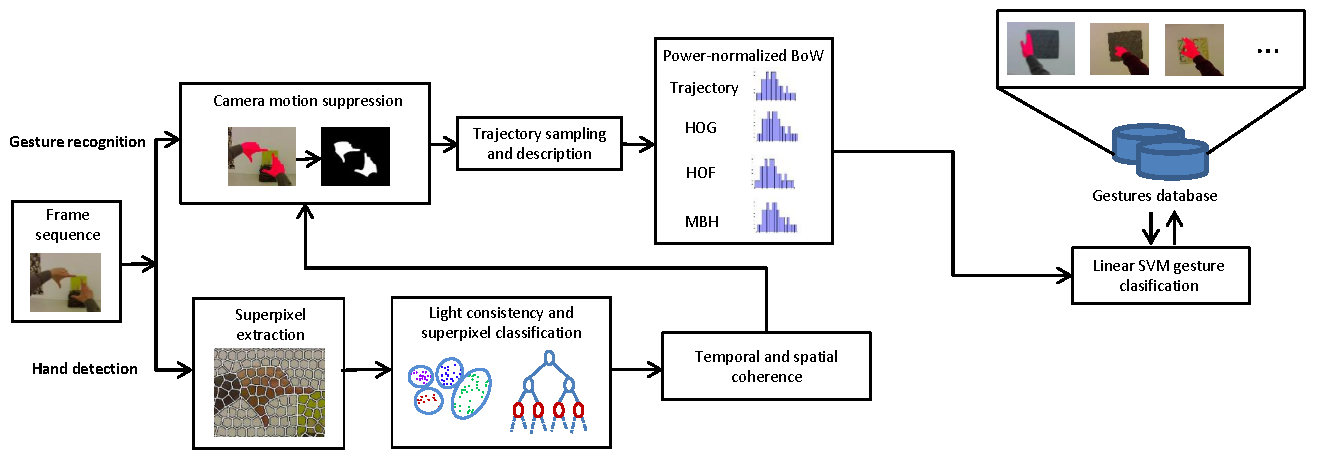
\includegraphics[width=\linewidth]{Figures/schema.pdf}
\caption{Outline of the proposed Gesture Recognition method.}
\label{schema}
\end{figure}
Gesture recognition systems should recognize both static and dynamic hand movements. Therefore, we propose to describe each gesture as a collection of dense trajectories extracted around hand regions. Feature points are sampled inside and around the user's hands and tracked during the gesture; then several descriptors are computed inside a spatio-temporal volume aligned with each trajectory, in order to capture its shape, appearance and movement at each frame. 
These descriptors are coded,  using the Bag of Words approach and power normalization, in order to obtain the final feature vectors, which are then classified using a linear SVM classifier. A summary of our approach is presented in Figure \ref{schema}.

In the next subsections we will introduce the main components of our approach: camera motion suppression, trajectory sampling and description, the power normalized Bag of Words and the final classification. We will also explain how these steps exploit the hand segmentation approach we have presented in the previous chapter.

\subsection{Feature points sampling}
We start by describing how we densely sample feature points for generating trajectories. To this aim, we consider a grid spaced by $W$ pixels. Sampling is carried out on each
spatial scale separately. This guarantees that feature points equally cover all spatial
positions and scales. Experimental results showed that a sampling step size of $W = 5$ pixels is dense
enough to give good results over all datasets. There are at most 8 spatial scales in total, depending on the
resolution of the video. The spatial scale increases by a factor of $1/\sqrt{2}$.
Our goal is to track all these sampled points through the video. However, in homogeneous image
areas without any structure, it is impossible to track any point. We remove points in these areas. Here, we
use the criterion that the points are removed if the eigenvalues of the auto-correlation
matrix are very small. We set a threshold $T$ on the eigenvalues for each frame $I$ as
\begin{equation}
T = 0.001 \times \max_{i\in I} \min(\lambda_i^1, \lambda_i^2)
\end{equation}

where $(\lambda_i^1, \lambda_i^2)$ are the eigenvalues of point $i$ in the image $I$. Experimental results showed that a value
of 0.001 represents a good compromise between saliency and density of the sampled points.

\subsection{Camera motion suppression}
A key step in our approach is to remove camera motion. To this end, the homography between two consecutive frames is estimated running the RANSAC algorithm on features points sampled as described. 

An homography (or \textit{projective transformation}) is defined by the following equation, where $x_1$ and $x_2$ are 2-d points expressed in homogeneous coordinates:
$$
x_1 = \left[\begin{array}{c c c}
 h_{11} & h_{12} & h_{13} \\
 h_{21} & h_{22} & h_{23} \\
 h_{31} & h_{32} & h_{33}
 \end{array}\right] x_2
$$
and, because two homography matrices that differ for a scale are equivalent, this matrix has only 8 degrees of freedom. RANSAC is accomplished to produce a good homography with the following steps:
\begin{enumerate}
\item Randomly selecting a subset of feature points
\item Fitting an homography to the selected subset
\item Determining the number of outliers
\item Repeating steps 1-3 for a prescribed number of iterations, and select the iteration with the minimum amount of outliers
\end{enumerate}

This would be the standard way to fit an homography between two frames. However, in first-person camera views hands movement is not consistent with camera motion and this generates wrong matches between the two frames. For this reason we introduce a segmentation mask that disregards feature matches belonging to hands. In fact, without the hand segmentation mask, many feature points from the user's hands would become inliers, degrading the homography estimation. As a consequence, the trajectories extracted from the video would be incorrect. Instead, computing an homography using feature points from non-hand regions allows us remove all the camera movements.

\subsection{Trajectory Sampling and description}
\label{trajectory-descr}
Having removed camera motion between two adjacent frames, trajectories can be extracted. The second frame is warped with the estimated homography, the optical flow between the first and the second frame is computed, and then feature points around the hands of the user are sampled and tracked following what \cite{wang:2011:inria-00583818:1} does for human action recognition.

Feature points are tracked on each spatial scale separately. For each frame $I_t$, its dense optical flow field
$\omega_t = (u_t, v_t)$ is computed w.r.t. the next frame $I_{t+1}$, where $u_t$ and $v_t$ are the horizontal and vertical
components of the optical flow. Given a point $P_t = (x_t, y_t)$ in frame $I_t$, its tracked position in frame $I_{t+1}$
is smoothed by applying a median filter on $\omega_t$:
\begin{equation}
P_{t+1} = (x_{t+1}, y_{t+1}) = (x_t, y_t) + (M * \omega_t)
\end{equation}
where $M$ is the median filtering kernel. The size of the median filter kernel $M$ is $3 \times 3$ pixels. As the
median filter is more robust to outliers than bilinear interpolation, it improves trajectories
for points at motion boundaries that would otherwise be smoothed out.
Once the dense optical flow field is computed, points can be tracked very densely without additional
cost. Another advantage of the dense optical flow is the smoothness constraints which allow relatively
robust tracking of fast and irregular motion patterns. To extract dense optical flow fields, we
use Farneback's algorithm \cite{farneback2003two} which embeds a translation motion model between neighborhoods of two consecutive
frames. Polynomial expansion is employed to approximate pixel intensities in the neighborhood.

Points of subsequent frames are concatenated to form trajectories: $(P_t,  P_{t+1}, P_{t+2}, ...))$. As trajectories
tend to drift from their initial locations during the tracking process, we limit their length to $L$ frames
in order to overcome this problem (based on our preliminary tests, we set $L=30$). For each frame, if no tracked point is found
in a $W \times W$ neighborhood, a new point is sampled and added to the tracking process so that a dense coverage
of trajectories is ensured.

As static trajectories do not contain motion information, we prune them in a post-processing stage.
Trajectories with sudden large displacements, most likely to be erroneous, are also removed. Such trajectories
are detected, if the displacement vector between two consecutive frames is larger than 70\% of the
overall displacement of the trajectory.

Furthermore, in contrast to what \cite{wang:2011:inria-00583818:1} does, trajectories are restricted to lie inside and around the user's hands: at each frame the hand mask is dilated, and all the feature points outside the computed mask are discarded.


Then, the spatio-temporal volume aligned with each trajectory is considered, and Trajectory descriptor, HOG, HOF and MBH are computed around it. The trajectory descriptors encodes local motion patterns. Given a trajectory of length $L$, we describe its
shape by a sequence $(\Delta P_t, ..., \Delta P_{t+L-1})$ of displacement vectors $\Delta P_t = (P_{t+1}- P_t) = (x_{t+1} -
xt, y_{t+1}- y_t)$. The resulting vector is normalized by the sum of displacement vector magnitudes:
\begin{equation}
T = \frac{(\Delta P_t, .., \Delta P_{t+L-1})}{\sum_{j=t}^{t+L-1} \| \Delta P_j \|}
\end{equation}
As we use trajectories with a fixed length of $L = 30$ frames, we obtain a 60 dimensional descriptor.

Besides the trajectory shape information, we also design descriptors to embed appearance and motion
information. We compute
descriptors within a space-time volume aligned with a trajectory to encode the motion information. The size of the volume is $N \times N$ pixels and $L$ frames long. To embed structure information, the volume is subdivided into a spatio-temporal grid of size $n_\sigma \times n_\sigma \times n_\tau$. We compute a descriptor (e.g.,
HOG, HOF or MBH) in each cell of the spatio-temporal grid, and the final descriptor is a concatenation
of these descriptors. The default parameters for our experiments are $N = 32$, $n_\sigma = 2$, $n_\tau = 3$.

As we have already said in Chapter \ref{chpt2}, HOG focuses on static appearance information, whereas HOF captures the
local motion information. We compute the HOG and HOF descriptors along the dense trajectories. For both HOG and HOF,
orientations are quantized into 8 bins with full orientation and magnitudes are used for weighting. An
additional zero bin is added for HOF (i.e., in total 9 bins). It accounts for pixels whose optical flow
magnitudes are lower than a threshold. Both descriptors are normalized with their $L_2$ norm. The final
descriptor size is 96 for HOG (i.e., $2\times 2\times 3\times 8$) and 108 for HOF (i.e., $2\times 2 \times 3 \times 9$).

The motion boundary histogram (MBH) descriptor computes derivatives separately for the horizontal and vertical components of the optical flow. The descriptor encodes the relative motion between pixels, and since MBH represents
the gradient of the optical flow, locally constant camera motion is removed and information about changes
in the flow field (i.e., motion boundaries) is kept. MBH is more robust to camera motion than optical flow,
and thus more discriminative.
We employ MBH s motion descriptor for trajectories. The MBH descriptor separates
optical flow $\omega = (u, v)$ into its horizontal and vertical components. Spatial derivatives are computed
for each of them and orientation information is quantized into histograms. The magnitude is used for
weighting. We obtain a 8-bin histogram for each component (i.e., MBHx and MBHy). Both histogram
vectors are normalized separately with their $L_2$ norm. The dimension is 96 (i.e., $2 \times 2 \times 3 \times 8$) for both
MBHx and MBHy.
For both HOF and MBH descriptor computation, we reuse the dense optical flow that is already
computed to extract dense trajectories.

While HOF and MBH are averaged on five consecutive frames, a single HOG descriptor is computed for each frame. In this way we can better describe how the hand pose changes in time. After this step, we get a variable number of trajectories for each gesture. In order to obtain a fixed size descriptor, the Bag of Words approach is exploited: we train four separate codebooks, one for each descriptor. Each codebook contains 500 visual words and is obtained running the $k$-means algorithm in the feature space. 

Since BoW histograms in our domain tend to be sparse, they are power normalized to unsparsify the representation, while still allowing for linear classification. To perform power-normalization \cite{perronnin2010improving}, the following function is applied to each bin $h_i$:
\begin{equation}
f(h_i) = \textrm{sign} (h_i) \cdot |h_i|^{\frac{1}{2}}
\end{equation}

We have also observed that power-normalization greatly improves the final accuracy. The feature vector is then obtained by the concatenation of its four power-normalized histograms. Eventually, gestures are recognized using a linear SVM 1-vs-1 classifier. SVM 1-vs-all and SVM Multiclass classifiers were also tested.

\section{Experimental Results}

We now evaluate the performance of the proposed approach. To compare the performance of our gesture recognition algorithm with existing approaches, we test it on the Cambridge-Gesture database \cite{kim2007tensor}, which includes nine hand gesture types performed on a table, under different illumination conditions. To better investigate the effectiveness of the proposed approach in videos taken from the ego-centric perspective and in a museum setting, we also propose two far more realistic and challenging dataset which contains seven gesture classes, performed by five subjects in an interactive exhibition room which functions as a virtual museum and in a real museum. 

The Cambridge Hand Gesture dataset contains 900 sequences of nine hand gesture classes. Although this dataset does not contain ego-vision videos it is useful to compare our results to recent gesture recognition techniques. In particular, each sequence is recorded with a fixed camera, placed over one hand, and hands perform leftward and rightward movements on a table, with different poses. The whole dataset is divided in five sets, each of them containing image sequences taken under different illumination conditions. The common test protocol, proposed in \cite{kim2007tensor}, requires to use the set with normal illumination for training and the remaining sets for testing, thus we use the sequences taken in normal illumination to generate the BoW codebooks and to train the SVM classifier. Then, we perform the test using the remaining sequences.   

Table \ref{cambridge} shows the recognition rates obtained with our gesture recognition approach, compared with the ones of tensor canonical correlation analysis (TCCA) \cite{kim2009canonical}, product manifolds (PM) \cite{lui2010action}, tangent bundles (TB) \cite{lui2011tangent} and spatio-temporal covariance descriptors (Cov3D) \cite{sanin2013spatio}. Results show that proposed method outperforms the existing state-of-the-art approaches.


\begin{table}
\begin{center}
\begin{tabular}{|l|c|c|c|c|c|}
\hline
\textbf{Method}					& \textbf{Set1}		& \textbf{Set2}		& \textbf{Set3}		& \textbf{Set4}	 	& \textbf{Overal}l \\
\hline
\hline
TCCA \cite{kim2009canonical}		& 0.81		& 0.81		& 0.78		& 0.86		& 0.82 \\
\hline
PM \cite{lui2010action}			& 0.89		& 0.86		& 0.89		& 0.87		& 0.88  \\
\hline
TB \cite{lui2011tangent}			& \textbf{0.93}	& 0.88		& 0.90		& 0.91		& 0.91 \\
\hline
Cov3D \cite{sanin2013spatio}		& 0.92		&\textbf{0.94}	& 0.94		& 0.93		& 0.93 \\
\hline
\textbf{Our method}			& 0.92		& 0.93		& \textbf{0.97}	& \textbf{0.95}	& \textbf{0.94} \\
\hline
\end{tabular}
\end{center}
\caption{Recognition rates on the Cambridge dataset.}
\label{cambridge}
\end{table}


\begin{figure}
\centering
\subfigure[\textit{Like} gesture in the \textit{museum} setting]{
  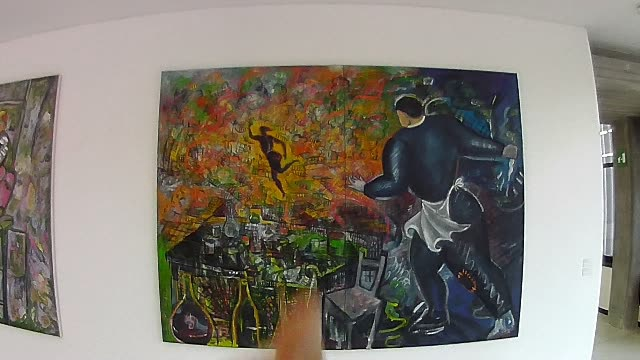
\includegraphics[width=0.2\linewidth]{Figures/like_16695_16718_all1.jpg}
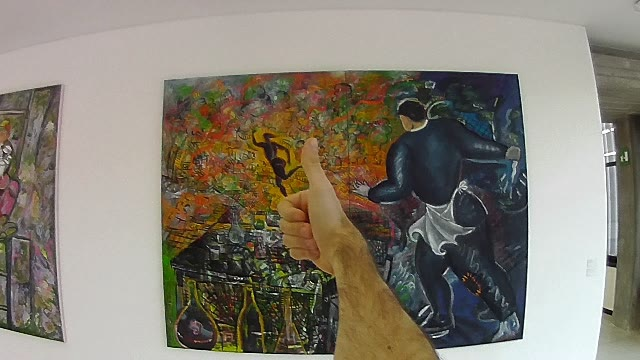
\includegraphics[width=0.2\linewidth]{Figures/like_16695_16718_all14.jpg}
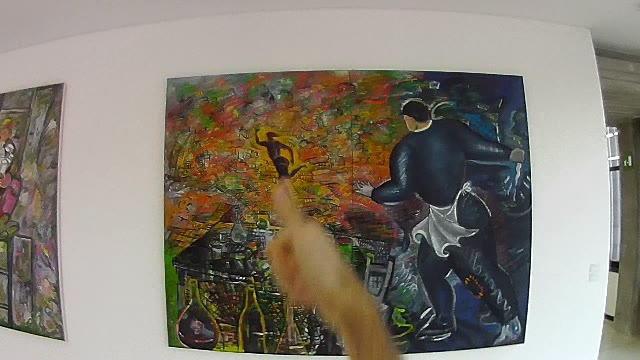
\includegraphics[width=0.2\linewidth]{Figures/like_16695_16718_all21.jpg}
}\\
\subfigure[\textit{Dislike} gesture]{
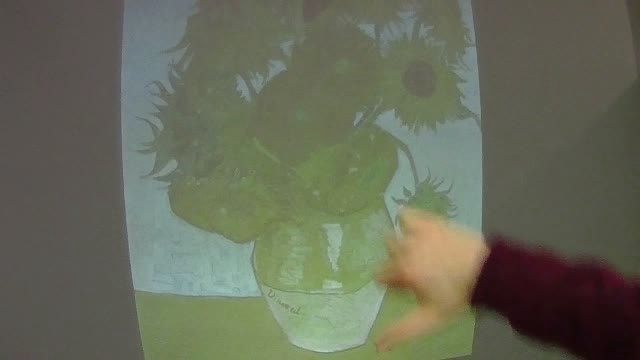
\includegraphics[width=0.2\linewidth]{Figures/dislike_10962_11000_all3.jpg}
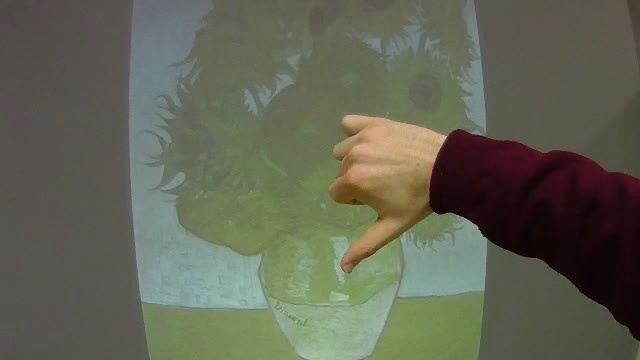
\includegraphics[width=0.2\linewidth]{Figures/dislike_10962_11000_all23.jpg}
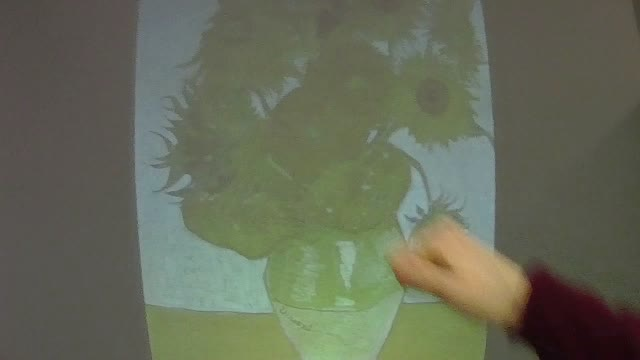
\includegraphics[width=0.2\linewidth]{Figures/dislike_10962_11000_all35.jpg}
}\\
\subfigure[\textit{Ok} gesture in the \textit{museum} setting, in low light]{
  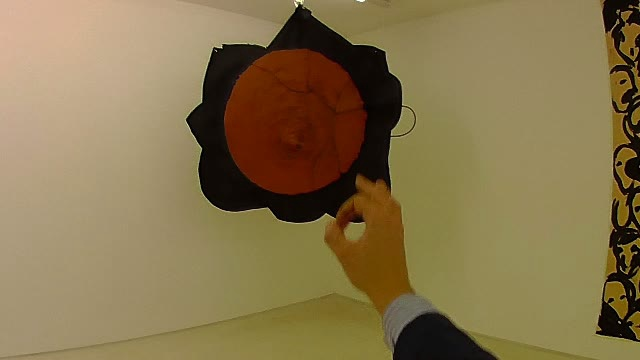
\includegraphics[width=0.2\linewidth]{Figures/ok_2696_2735_all5.jpg}
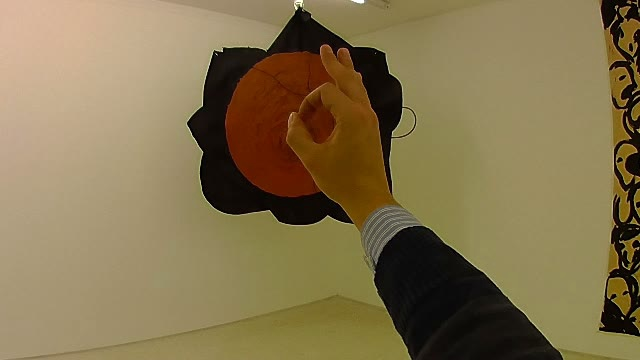
\includegraphics[width=0.2\linewidth]{Figures/ok_2696_2735_all23.jpg}
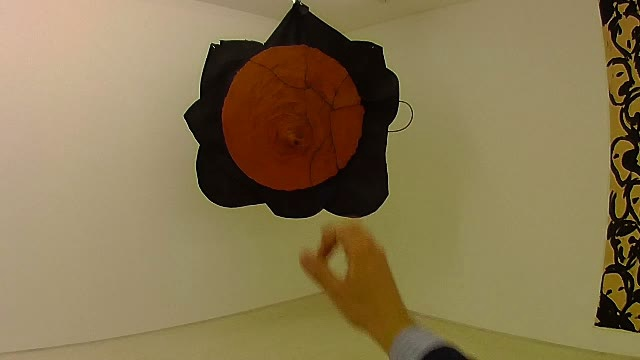
\includegraphics[width=0.2\linewidth]{Figures/ok_2696_2735_all36.jpg}
}\\
\subfigure[\textit{Point} gesture]{
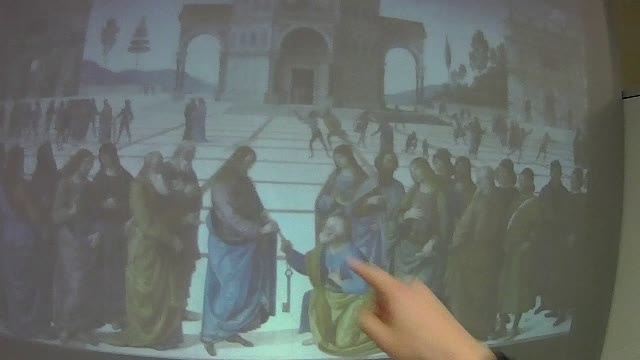
\includegraphics[width=0.2\linewidth]{Figures/point_4624_4654_all3.jpg}
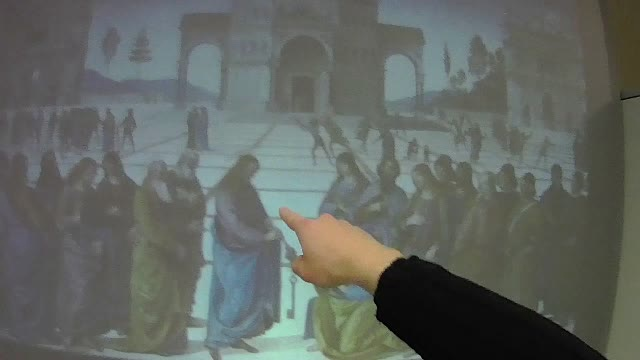
\includegraphics[width=0.2\linewidth]{Figures/point_4624_4654_all8.jpg}
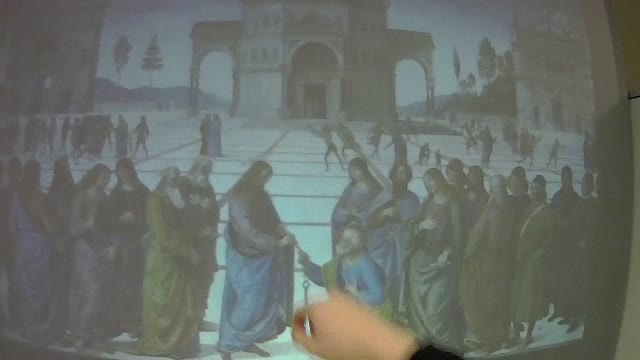
\includegraphics[width=0.2\linewidth]{Figures/point_4624_4654_all28.jpg}
}\\
\subfigure[\textit{Slide right to left} gesture in the \textit{museum} setting, while another visitor walks in]{
  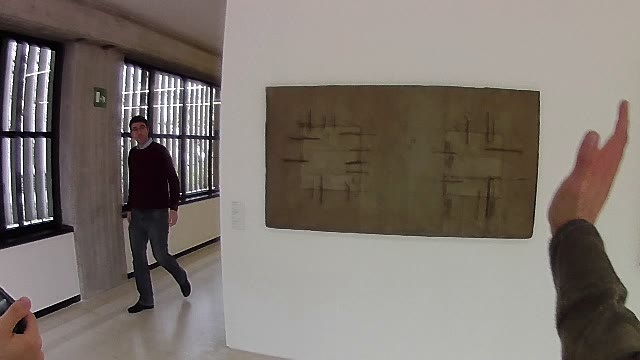
\includegraphics[width=0.2\linewidth]{Figures/slide_2_7348_7383_all12.jpg}
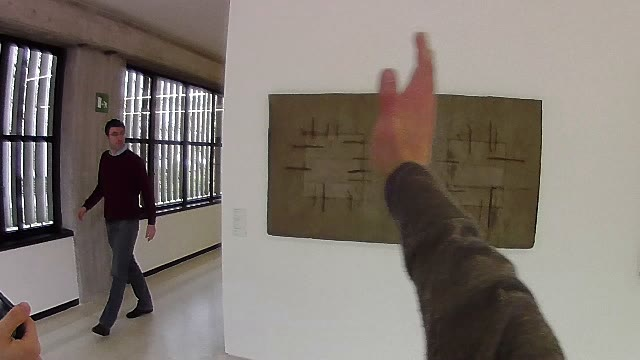
\includegraphics[width=0.2\linewidth]{Figures/slide_2_7348_7383_all20.jpg}
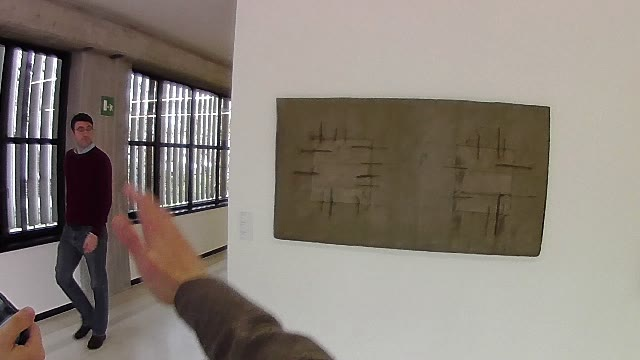
\includegraphics[width=0.2\linewidth]{Figures/slide_2_7348_7383_all30.jpg}
}\\
\subfigure[\textit{Slide left to right} gesture in the \textit{demo room} setting performed by user 3]{
  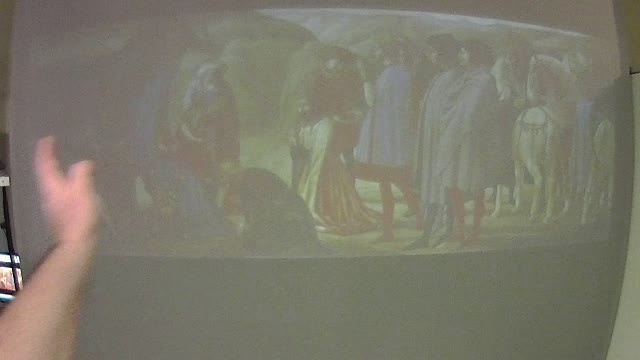
\includegraphics[width=0.2\linewidth]{Figures/slide_2_2030_2058_all7.jpg}
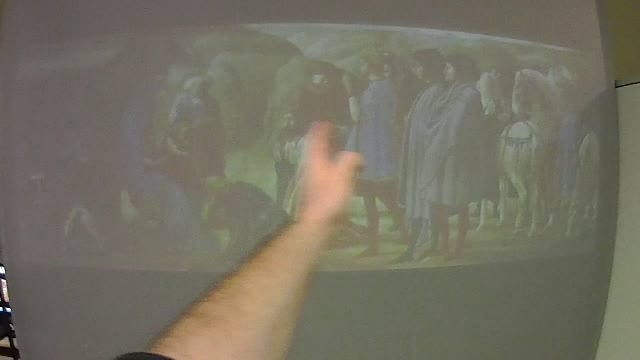
\includegraphics[width=0.2\linewidth]{Figures/slide_2_2030_2058_all14.jpg}
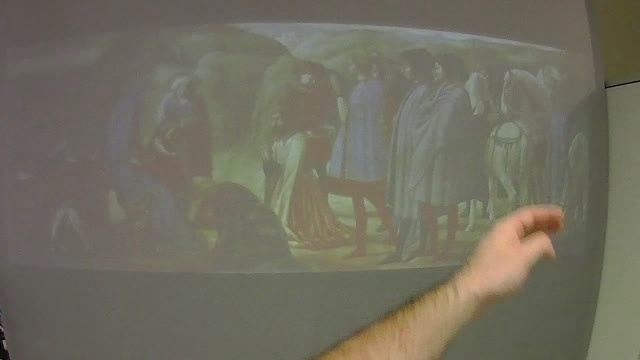
\includegraphics[width=0.2\linewidth]{Figures/slide_2_2030_2058_all23.jpg}
}\\
\subfigure[\textit{Take a picture} gesture in the \textit{demo room} setting]{
  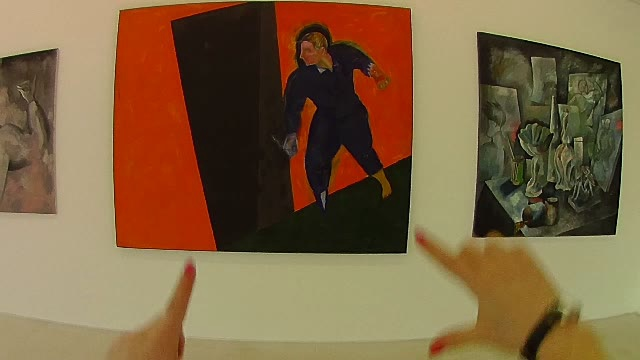
\includegraphics[width=0.2\linewidth]{Figures/take_a_picture_23956_24002_all2.jpg}
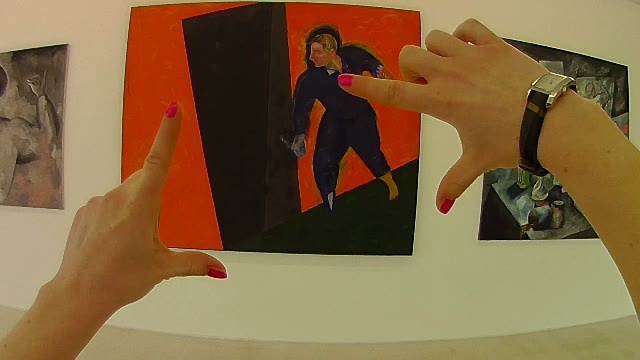
\includegraphics[width=0.2\linewidth]{Figures/take_a_picture_23956_24002_all25.jpg}
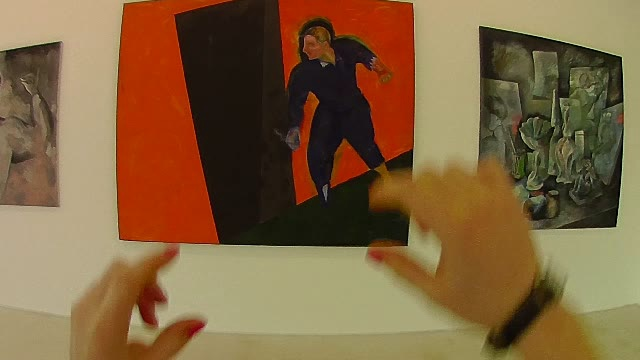
\includegraphics[width=0.2\linewidth]{Figures/take_a_picture_23956_24002_all43.jpg}
}
\caption{Sample gestures from the \datasetunimore{} dataset and the Maramotti dataset.}
\label{example-unimore}
\end{figure}

We then propose the \datasetunimore{} dataset, a gesture recognition dataset taken from the ego-centric perspective in a virtual museum environment. It consists of 700 video sequences, all shot with a wearable camera, in an interactive exhibition room, in which paintings and artworks are projected over a wall, in a virtual museum fashion (see figure \ref{example-unimore}). The camera is placed on the user's head and captures a 800 $\times$ 450, 25 frames per second 24-bit RGB image sequence. In this setting, five different users perform seven hand gestures: \textit{like}, \textit{dislike}, \textit{point}, \textit{ok}, \textit{slide left to right}, \textit{slide right to left} and \textit{take a picture}. Some of them (like the \textit{point}, \textit{ok}, \textit{like} and \textit{dislike} gestures) are statical, others (like the two \textit{slide} gestures) are dynamical. 
This dataset is very challenging since there is fast camera motion and users have not been trained before recording their gestures, so that each user performs the gestures in a slightly different way, as would happen in a realistic context. We have publicly released our dataset\footnote{\url{http://imagelab.ing.unimore.it/files/ego_virtualmuseum.zip}}.

%In the demo room setting, users perform gestures in front of a wall over which the works of art are projected. This setting is quite controlled: the illumination is constant, the art works are in low light, while hands are well illuminated. In the same way, in the \textit{museum} setting, users perform gestures in front of real artworks inside a museum. This is a realistic and very challenging environment: the illumination changes, other visitors are present and sometimes walk in. 
Since Ego Vision applications are highly interactive, their setup step must be fast (i.e. few positive examples can be acquired). Therefore, to evaluate the proposed gesture recognition approach, we train a 1-vs-1 linear classifier for each user using only two randomly chosen gestures per class as training set. The reported results are the average over 100 independent runs.

In Table \ref{gesture_comparison} we show the gesture recognition accuracy for each of the five subjects, and we also compare with the ones obtained without the use of the hand segmentation mask for camera motion removal and trajectories pruning.  Results show that our approach is well suited to recognize hand gestures in the ego-centric domain, even using only two positive samples per gesture, and that the use of the segmentation mask can improve recognition accuracy.


\begin{table}
\begin{center}
\renewcommand{\arraystretch}{1.3}
\centering
\begin{tabular}{|l|c|c|}
\hline
\textbf{User}							& \textbf{No segmentation} & \textbf{With segmentation}  \\
\hline
\hline
Subject 1				 			& 0.91 		& \textbf{0.95} \\
\hline
Subject 2			 				& 0.87 		& \textbf{0.87} \\
\hline
Subject 3					 		& 0.92		& \textbf{0.95}\\
\hline
Subject 4							& \textbf{0.96}	& 0.94 \\
\hline
Subject 5							& 0.91		& \textbf{0.96} \\
\hline
Average						&  0.91	& \textbf{0.93}  \\
\hline
\end{tabular}
\end{center}
\caption{Gesture recognition accuracy on the \datasetunimore{} dataset with and without hand segmentation.}
\label{gesture_comparison}
\end{table}

On a different note, to test our approach in a real setting, we created a dataset with videos taken in the Maramotti modern art museum, in which paintings, sculptures and \textit{objets d'art} are exposed. As in the previous dataset, the camera is placed on the user's head and captures a 800 $\times$ 450, 25 frames per second image sequence. The Maramotti dataset contains 700 video sequences, recorded by five different persons (some are the same of the Interactive Museum dataset), each performing the same gestures as before in front of different artworks. We have publicly released this dataset too\footnote{\url{ http://imagelab.ing.unimore.it/files/ego_maramotti.zip}}.
   
Figure \ref{example-unimore} show some examples of gestures performed in the two datasets. In the Interactive Museum dataset, users perform gestures in front of a wall over which the works of art are projected. This setting is quite controlled: the illumination is constant, the art works are in low light, while hands are well illuminated. On the other hand, in the Maramotti dataset, users perform gestures in front of real artworks inside a museum. This is a realistic and very challenging environment: the illumination changes, other visitors are present and sometimes walk in. In both cases there is significant camera motion, because the camera moves as the users move their heads or arms. It is also important to underline that users have not been trained before recording their gestures, so each user performs the gestures in a slightly different way, as would happen in a realistic context.  

In Table \ref{gesture_comparison_maramotti} we show the results of our gesture recognition approach on the Maramotti dataset. As can be seen, in this case the challenging and real environment causes a drop in accuracy. This is mainly due to the illumination changes, to the presence of other visitors, and to the fact that often the artworks are better illuminated than hands.
Since our wearable vision devices is fully connected to a central server, we show how the use of other visitors' gestures can improve the recognition accuracy.
In our scenario each visitor coming to the museum performs, in the initial setup phase, two training gestures for each class. These training gestures from past visitors, manually checked, are used to augment the training set, so no erroneous data is accumulated into the model. In particular, in our test ``Augmented'' (Table \ref{gesture_comparison_maramotti}) each ego-vision wearable device uses two randomly chosen gestures performed by its user as training, plus gestures performed by the remaining four users supplied by their devices to the central server. Results show that this distributed approach is effective and leads to a significant improvement in accuracy.


\begin{table}[tb]
\renewcommand{\arraystretch}{1.3}
\caption{Gesture recognition accuracy on the Maramotti dataset.}
\label{gesture_comparison_maramotti}
\centering
\begin{tabular}{|l|c|c|}
\hline
\textbf{User}					& \textbf{Single user's Gestures} 	& \textbf{Augmented}  \\
\hline
\hline
User A						& 0.54 			& \textbf{0.65} \\		% 4 Beppe
\hline
User B			 				& 0.52 			& \textbf{0.72} \\		% 2 Francesco
\hline
User C			 			& 0.68 			& \textbf{0.68} \\		% 1 Lorenzo
\hline
User F					 		& 0.56 			& \textbf{0.79} \\		% 3 Stefano
\hline
User G						& 0.53 			& \textbf{0.72} \\		% 5 Michela
\hline
\textbf{Average}					& 0.57	  		& \textbf{0.71} \\
\hline
\end{tabular}
\end{table}

We described a novel approach to cultural heritage fruition based on ego-centric vision devices. Our work is motivated by the increasing interest in ego-centric vision and by the growth of the cultural market, which encourages the development of new interfaces to interact with the cultural heritage. We presented a gesture and painting recognition model that can deal with static and dynamic gestures and can benefit from a distributed training. Our gesture recognition and hand segmentation results outperform the state-of-the-art approaches on Cambridge Hand Gesture and CMU EDSH datasets. Finally, we ran an extensive performance analysis of our system on a wearable board. 

In the next chapter, a real-time version of the described algorithm will be proposed, and we will describe the necessary optimizations steps to make such implementation real-time.